%! TeX program = lualatex
\documentclass[../main.tex]{subfiles}
\begin{document}
\begin{lesson}{Tangent lines and derivatives (at a fixed number)}

  A balloon moves in a straight line. Its position function \(s(t)\) with respect to time \(t\) is sketched below. 

  \begin{center}
    \includegraphics{../standalones/build/plot_tangent_exercise}
  \end{center}

  Fix a constant \(a\), say \(a = 1\), in the interval \([0,2]\). Suppose \(b\) is in \([0,2]\), explain the physical interpretation of the following. 

  \(\frac{s(b) - s(a)}{b - a}\)
  \blanklines{5}

  Explain the physical interpretation of its limit as \(t \to a\) to someone who has never learned calculus. 

  \(\lim_{t \to a} \frac{s(t) - s(a)}{t - a}\)
  \blanklines{10}

  Motivated by the above example, the \hlmain{tangent line to (a generic function) \(f(x)\) at \(a\)} is \underline{\hspace{2cm}} line passing through \underline{\hspace{2in}} and having slope 
  \blanklines{5}
  \clearpage

  \begin{mdframed}[style=simple]
    Let \(f(x)\) be a function defined on an \underline{\hspace{1in}} interval containing \(a\). The \hlmain{derivative of \(f(x)\) at \(a\)}, denoted by \hlmain{\(f'(a)\)} is defined by
    \begin{equation}\label{eq:def-derivative-1}
      %
    \end{equation}
    or equivalently 
    \begin{equation}\label{eq:def-derivative-2}
      %
    \end{equation}
    provided that \underline{\hspace{2in}}.

  \end{mdframed}

  \faStar{} Geometrically, \(f'(a)\) is \underline{\hspace{5in}}.

  Terminologies. 
  \begin{itemize}
    \item If \(f'(a)\) exists, then \(f\) is said to be \hlmain{differentiable at \(a\)}.
    \item If \(f'(a)\) does not exist, then \(f\) is said to be \hlmain{not differentiable at \(a\)}.
  \end{itemize}

  \bigskip
  \begin{example}
    Find the derivative of \(x^{2}\) at \(3\) using Equation~\eqref{eq:def-derivative-1} and \eqref{eq:def-derivative-2}. Write down the equation of the tangent line at \(x = 3\).

    \blanklines{30}
  \end{example}
  \clearpage

  \begin{example}
    Sketch a function \(f(x)\) whose derivative at \(-1\) does not exist. Explain why your answer is correct.

    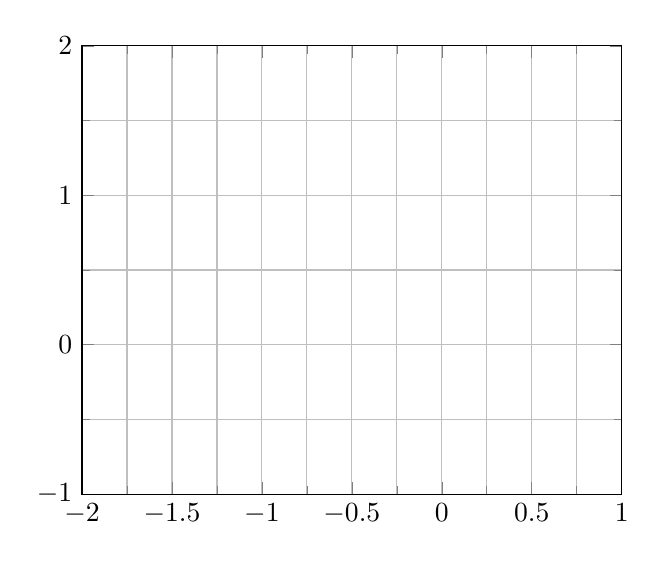
\begin{tikzpicture}[scale=1]
      \begin{axis}[xmin=-2, xmax=1, ymin=-1, ymax=2, grid=both, minor tick num=1]

      \end{axis}
    \end{tikzpicture}
  \end{example}

  \begin{example}
    Use Equation~\eqref{eq:def-derivative-1} or \eqref{eq:def-derivative-2} to show \(y = |x|\) does not have a derivative at \(0\).
    \blanklines{10}
  \end{example}

  \begin{example}[\href{https://www.youtube.com/watch?v=yrc632oilWo}{The slingshot}]
    Consider \(f(x) = \begin{cases} x^{2} &\text{if } x \le 2\\ 4x - 4& \text{if } x > 2 \end{cases}\). Does \(f'(2)\) exist? 

    \blanklines{20}
  \end{example}
  \clearpage

  \bigskip
  \begin{example}
    Sketch a function satisfying \(f'(2) = 2\) and \(f'(3) = -1\) and \(f(2) = 1\). Sketch \(f\).
    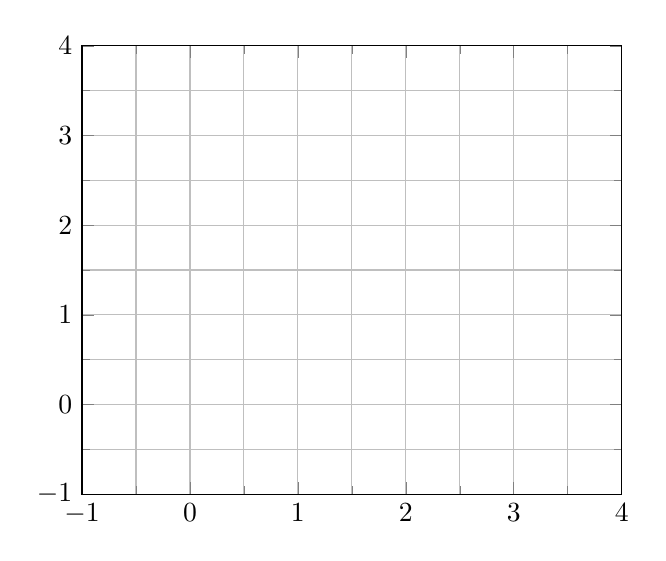
\begin{tikzpicture}[scale=1]
      \begin{axis}[xmin=-1, xmax=4, ymin=-1, ymax=4, grid=both, minor tick num=1]

      \end{axis}
    \end{tikzpicture}
  \end{example}
  \begin{example}
    Find the derivative of \(f(x) = 3x^{2} - x\) at \(2\) from the definition. Write down the equation for the tangent line to \(y = f(x)\) at the point \((2, f(2))\).

    \blanklines{30}
  \end{example}

\end{lesson}
\end{document}

